\documentclass[12pt]{article}
\usepackage{fontspec}            % шрифты
    \setmainfont{Times New Roman}
    \setmonofont{Courier New}
\usepackage[english,russian]{babel}
\usepackage{ragged2e}            % для выравнивания по ширине, по центру
    \justifying
    \sloppy
\usepackage{indentfirst}         % отступы первой строки
    \setlength{\parindent}{12.5mm}
\usepackage{setspace}            % межстрочный интервал полтора
    \onehalfspacing
\usepackage{geometry}     
    \geometry{                   % установление границ документа
        a4paper,
        left=30mm,
        right=15mm,
        top=25mm,
        bottom=25mm
    }
\usepackage{fancyhdr}            % нумерация страниц справа снизу
    \pagestyle{fancy}
    \renewcommand{\headrulewidth}{0pt}
    \fancyhf{}
    \fancyfoot[R]{\thepage}
\usepackage[]{graphicx}          % вставка картинок
\usepackage{float}
\usepackage{hyperref}            % для перехода из содержания к разделам по главам
\usepackage{tocloft}             % управление настройками содержания
\usepackage{listings}            % для листинга
\usepackage{enumitem}            % для сдвига списков вправо
    \setlist[itemize]{noitemsep,leftmargin=2cm}
\usepackage{amsmath}             % для математических символов
\usepackage{tabularx}            % работа с таблицами
\usepackage{longtable}       
\usepackage{seqsplit}            % для свободного переноса длинных строк кода
\usepackage{lscape}              % для альбомной ориентации страниц
\usepackage[none]{hyphenat}      % предотвращение переноса через тире         
\usepackage{pdflscape}           % для переворота страниц pdf
\usepackage{caption}             % для работы с подписями, чтобы удалить лишние <:>
    \captionsetup[table]{labelsep=space}

% стиль текста "код"
\newcommand{\code}[1]{\fontsize{10pt}{12pt}\texttt{#1}}


\begin{document}

\begin{titlepage}

\newpage
\fontsize{14pt}{16pt}\selectfont
\begin{center}
    \textbf{МИНИСТЕРСТВО НАУКИ И ВЫСШЕГО ОБРАЗОВАНИЯ РОССИЙСКОЙ ФЕДЕРАЦИИ}

    ФЕДЕРАЛЬНОЕ ГОСУДАРСТВЕННОЕ БЮДЖЕТНОЕ ОБРАЗОВАТЕЛЬНОЕ УЧРЕЖДЕНИЕ

    ВЫСШЕГО ОБРАЗОВАНИЯ

    «МОСКОВСКИЙ АВИАЦИОННЫЙ ИНСТИТУТ

    (национальный исследовательский университет)» (МАИ)

    \vspace{1cm}
    Кафедра 703

    \vspace{1cm}
    Курсовая работа

    по курсу «Технологии разработки программного обеспечения»

    Вариант № 3
\end{center}

\vspace{1cm}
\hfill
\begin{minipage}{0.4\textwidth}

    \raggedright

    Выполнил студент \\
    группы М7О-406С-21 \\
    Плужник\,В.М. \\
    \vspace{0.5cm}
    \rule{5cm}{0.4pt} \\

    Принял \\
    Барчев\,Н.Б. \\
    \vspace{0.5cm}
    \rule{5cm}{0.4pt} \\

    Дата сдачи лабораторной работы \\
    \vspace{0.5cm}
    \rule{5cm}{0.4pt} \\

\end{minipage}

\vfill
\begin{center}
    МОСКВА – 2025
\end{center}

\end{titlepage}
\renewcommand{\contentsname}{Содержание} % название содержания
\renewcommand{\cftsecpagefont}{}         % избавление от жирности текста
\renewcommand{\cftsecfont}{}             % избавление от жирности текста

\let\oldtableofcontents\tableofcontents  % сохранение нумерации
\renewcommand{\tableofcontents}{
    \oldtableofcontents
    \thispagestyle{fancy}
}

\tableofcontents

\newpage
\label{sec:task}
\section{Задание}

Составить описание класса для объектов-векторов, задаваемых координатами концов в трехмерном пространстве. Обеспечить операции сложения и вычитания векторов с получением нового вектора (суммы или разности), вычисления скалярного произведения двух векторов, длины вектора, косинуса угла между векторами.
\label{sec:pseudocode}
\section{Псевдокод}

\fontsize{8pt}{10pt}\selectfont
\begin{verbatim}

класс Вектор
{
    x, y, z

    операцияСложения(другой_вектор)
    операцияВычитания(другой_вектор)
    скалярноеУмножение(другой_вектор)
    векторноеУмножение(другой_вектор)
    длина()
    косинусМежду(другой_вектор)
    уголМежду(другой_вектор)
}

Вектор::операцияСложения(другой_вектор)
{
    новый = Вектор()
    новый.x = этот.x + другой_вектор.x
    новый.y = этот.y + другой_вектор.y
    новый.z = этот.z + другой_вектор.z
    вернуть новый
}

Вектор::операцияВычитания(другой_вектор)
{
    новый = Вектор()
    новый.x = этот.x - другой_вектор.x
    новый.y = этот.y - другой_вектор.y
    новый.z = этот.z - другой_вектор.z
    вернуть новый
}

Вектор::векторноеУмножение(другой_вектор)
{
    новый = Вектор()
    новый.x = этот.y * другой_вектор.z - этот.z * другой_вектор.y
    новый.y = этот.z * другой_вектор.x - этот.x * другой_вектор.z
    новый.z = этот.x * другой_вектор.y - этот.y * другой_вектор.x
    вернуть новый
}

Вектор::скалярноеУмножение(другой_вектор)
{
    результат = 0
    результат += этот.x * другой_вектор.x
    результат += этот.y * другой_вектор.y
    результат += этот.z * другой_вектор.z
    вернуть результат
}

Вектор::длина()
{
    результат = 0
    результат += этот.x * этот.x
    результат += этот.y * этот.y
    результат += этот.z * этот.z
    вернуть кореньИз(результат)
}

Вектор::косинусМежду(другой_вектор)
{
    вернуть этот.скалярноеУмножение(другой_вектор) / этот.длина() / другой_вектор.длина()
}

Вектор::уголМежду(другой_вектор)
{
    вернуть арккосинус(этот.косинусМежду(другой_вектор))
}

\end{verbatim}
\label{sec:info}
\section{Сведения о программной реализации}

\label{subsec:coding_env}
\subsection{Язык программирования и среда разработки}

При разработке применялись:
\begin{itemize}
    \item Компилятор MinGW 8.1.0
    \item Компоновщик Make 4.4.1
    \item Среда разработки Qt Creator 5.15.0
    \item Стандарт языка ISO C++ 17 Standard
\end{itemize}


\label{subsec:input_output}
\subsection{Входные и выходные данные}

Входные данные:
\begin{itemize}
    \item координаты \textit{(x,y,z)} векторов \textbf{a} и \textbf{b} в вещественном виде.
\end{itemize}

Выходные данные:
\begin{itemize}
    \item координаты \textit{(x,y,z)} вектора суммы \textbf{a+b};
    \item координаты \textit{(x,y,z)} вектора разности \textbf{a-b};
    \item координаты \textit{(x,y,z)} вектора векторного произведения \textbf{a$\times$b};
    \item косинус угла между между векторами \textbf{a} и \textbf{b};
    \item угол между векторами \textbf{a} и \textbf{b};
    \item длина вектора суммы \textbf{|a+b|};
    \item длина вектора разности \textbf{|a-b|};
    \item скалярное произведение векторов \textbf{a} и \textbf{b}.
\end{itemize}


\label{subsec:list_of_modules}
\subsection{Список спроектированных программных единиц}

{
    \setlength{\parindent}{0pt}
    \begin{table}[h!]
        \begin{tabularx}{\textwidth}{ |X|X|X| }
            
        \hline
        Класс&
        Назначение &
        Поля \\ \hline

        \multicolumn{3}{|c|}{Заголовочный файл mathVector.h} \\ \hline

        \code{class MathVector} &
        Предназначен для хранения координат вершины вектора и выполнение операций над вектором. &
        \code{float x, y, z}  - координаты вершины вектора. \\ \hline

        \end{tabularx}
    \end{table}
}

\newpage

{
    \setlength{\parindent}{0pt}
    \begin{table}[h!]
        \begin{tabularx}{\textwidth}{ |>{\raggedright\arraybackslash}X|>{\raggedright\arraybackslash}X|>{\raggedright\arraybackslash}X| }
            
        \hline
        Структура &
        Назначение &
        Поля \\ \hline

        \multicolumn{3}{|c|}{Заголовочный файл progRes.h} \\ \hline

        \code{struct Calculations} &
        Предназначена для хранение результатов операций между векторами. &
        \code{MathVector A, B} - вводимые векторы A и B\newline
        \code{MathVector Sum, Diff, CrossProd} - векторы суммы, разности и векторного произведения\newline
        \code{float cosines} - значения косинуса\newline
        \code{float angle} - значение угла между векторами\newline
        \code{float sumLength} - длина вектора суммы\newline
        \code{float diffLength} - длина вектора разности\newline
        \code{float dotProd} - значение скалярного произведения \\ \hline

        \end{tabularx}
    \end{table}
}

\newpage

\begin{landscape}
    \setlength{\parindent}{0pt}
    
    \begin{longtable}{ |>{\raggedright\arraybackslash}p{6cm}|>{\raggedright\arraybackslash}p{6cm}|>{\raggedright\arraybackslash}p{5cm}|>{\raggedright\arraybackslash}p{5cm}| }
    
    \hline
    Функция &
    Назначение &
    Возвращаемое/изменяемое значение &
    Параметры \\ \hline
    \endhead
    
    \hline
    \endfoot
    
    \multicolumn{4}{|c|}{Заголовочный файл mathVector.h} \\ \hline

    \code{\seqsplit{MathVector\newline MathVector::operator+(MathVector const\& obj)}} &
    Сложения векторов по координатам &
    Возвращает вектор \code{[MathVector]} суммы векторов &
    \code{MathVector\ const\&\ obj} - вектор для сложения \\ \hline
    
    \code{\seqsplit{MathVector\newline MathVector::operator-(MathVector\ const\&\ obj)}} &
    Вычитание векторов по координатам &
    Возвращает вектор \code{[MathVector]} разности векторов &
    \code{MathVector\ const\&\ obj} - вектор для вычитания \\ \hline

    \code{\seqsplit{MathVector\newline MathVector::crossProd(MathVector\ const\&\ obj)}} &
    Векторное умножение векторов &
    Возвращает вектор \code{[MathVector]} векторного произведения векторов &
    \code{MathVector\ const\&\ obj} - вектор для умножения. \\ \hline

    \code{\seqsplit{float\newline MathVector::dotProd(MathVector\ const\&\ obj)\ const}} &
    Вычисление скалярного произведения векторов &
    Возвращает значение скалярного произведения \code{[float]}. &
    \code{MathVector\ const\&\ obj} - вектор для произведения. \\ \hline

    \code{\seqsplit{float\ MathVector::len()}} &
    Определения длины вектора &
    Значение длины вектора \code{[float]}. &
    - \\ \hline

    \code{\seqsplit{float\newline MathVector::cosBetween(MathVector\ const\&\ obj)\ const}} &
    Определения косинуса между векторами. &
    Возвращает значение косинуса \code{[float]} между векторами. &
    \code{MathVector\ const\&\ obj} - вектор, между которым определяется косинус угла. \\ \hline

    \code{\seqsplit{float\newline MathVector::angle(MathVector\ const\&\ obj)\ const}} &
    Определения угла между векторами. &
    Возвращает значение угла  \code{[float]} в радианах между векторами. &
    \code{MathVector\ const\&\ obj} - вектор, между которым определяется угол. \\ \hline

    \code{\seqsplit{MathVector::MathVector(float\ xParam,\ float\ yParam,\ float\ zParam)}} &
    Конструктор по умолчанию. &
    - &
    \code{float xParam, float yParam, float zParam} - координаты вершины вектора (x,y,z) для инициализации вектора. \\ \hline

    \code{\seqsplit{MathVector::MathVector(MathVector \&copy)}} &
    Конструктор копирования. &
    - &
    \code{MathVector \&copy} - вектор для копирования. \\ \hline

    \multicolumn{4}{|c|}{Заголовочный файл mainwindow.h} \\ \hline

    \code{\seqsplit{void\ MainWindow::on\_calculate\_clicked()}} &
    Вычисление данных по нажатию клавиши. &
    - &
    - \\ \hline

    \end{longtable}
\end{landscape}
\label{sec:list_of_errors}
\section{Список диагностических сообщений с указанием возможных причин их возникновения}
{

    \setlength{\parindent}{0pt}
    
    \begin{longtable}{ |>{\raggedright\arraybackslash}p{0.3\textwidth}|>{\raggedright\arraybackslash}p{0.3\textwidth}|>{\raggedright\arraybackslash}p{0.3\textwidth}| }

    \hline
    Диагностическое сообщение &
    Причина появления &
    Возможное решение \\ \hline
    \endhead

    Не существует (в полях косинуса и угла) &
    Один из векторов является нулевым, все его координаты равны нулю &
    Ввести вместо нулевого вектора любой другой вектор \\ \hline

    \end{longtable}
}

\label{sec:instruction}
\section{Инструкция пользователя}

\begin{enumerate}
    
    \begin{figure}[H]
        \item Запустите программу.
        \vspace{0.3cm}
        

        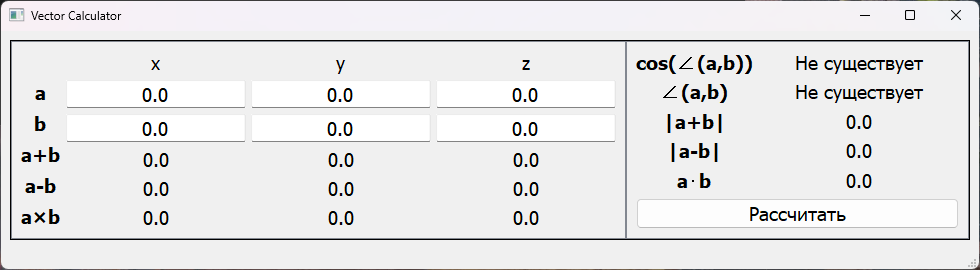
\includegraphics[width=\textwidth]{img//instruction1}
        \caption{}
    \end{figure}

    
    \begin{figure}[H]
        \item Введите желаемые значения координат векторов.
        \vspace{0.3cm}


        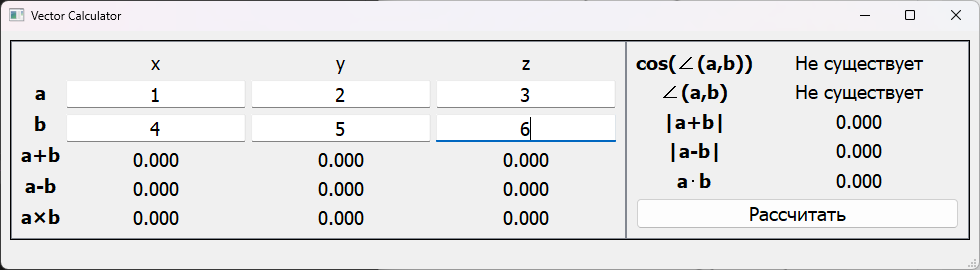
\includegraphics[width=\textwidth]{img//instruction2}
        \caption{}
    \end{figure}


    \begin{figure}[H]
        \item Нажмите кнопку <Рассчитать> и получить значение желаемой величины.
        \vspace{0.3cm}


        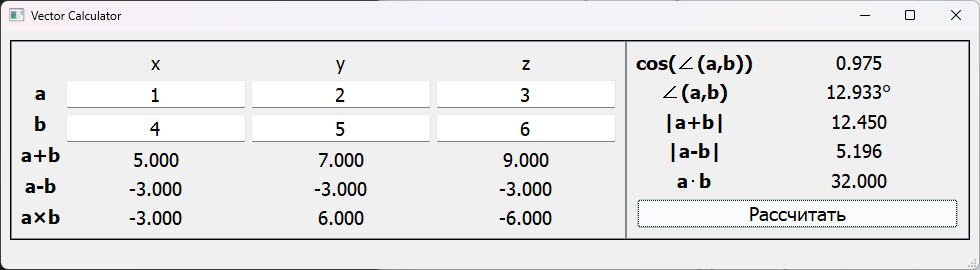
\includegraphics[width=\textwidth]{img//instruction3}
        \caption{}
    \end{figure}

\end{enumerate}
\begin{landscape}

\pagestyle{fancy}
\renewcommand{\headrulewidth}{0pt}
\setlength{\headheight}{17pt}
\fancyhf{}
\fancyhead[R]{\rotatebox{90}{\thepage}}

\label{sec:listing}
\section{Листинг программной разработки}

\lstset{
    basicstyle=\ttfamily\fontsize{10pt}{12pt}\selectfont,
    keepspaces=true,
    tabsize=4,
    breaklines=true,
    breakatwhitespace=true
}

\captionsetup[lstlisting]{labelformat=empty}


\begin{lstlisting}[caption={mathVector.h}]

#ifndef MATHVECTOR_H
#define MATHVECTOR_H

#include <cmath>

class MathVector
{
public:
    // Координаты вектора
    float x, y, z;

    // Математические операции для работы с векторами
    // Операции, которые возвращают векторные значения
    MathVector operator+(MathVector const& obj);   // операция сложения
    MathVector operator-(MathVector const& obj);   // операция вычитания
    MathVector crossProd(MathVector const& obj);   // операция векторного умножения
    // Операции, которые возвращают скалярные значения
    float dotProd(MathVector const& obj) const;    // операция скалярного умножения
    float len() const;                             //
    float cosBetween(MathVector const& obj) const; // операция определения косинуса между векторами
    float angle(MathVector const& obj) const;      // операция определения угла между векторами

    // Конструкторы
    MathVector(float xParam = 0, float yParam = 0, float zParam = 0);
    MathVector(MathVector &copy);
};

#endif // MATHVECTOR_H

\end{lstlisting}

\newpage
\begin{lstlisting}[caption={progRes.h}]

#ifndef PROGRES_H
#define PROGRES_H

#include <mathVector.h>

// Структура для хранения вводимых данных пользователем и результатов вычислений
struct Calculations
{
    MathVector A, B; // Векторы A и B
    MathVector       // Векторы суммы, разности и векторного произведения
        Sum,
        Diff,
        CrossProd;
    float
        cosines,     // значения косинуса
        angle,       // значение угла между векторами
        sumLength,   // длина вектора суммы
        diffLength,  // длина вектора разности
        dotProd;     // значение скалярного произведения

    Calculations();
};

#endif // PROGRES_H

\end{lstlisting}

\newpage
\begin{lstlisting}[caption={mainwindow.h}]

#ifndef MAINWINDOW_H
#define MAINWINDOW_H

#include <QMainWindow>
#include <QLineEdit>
#include <QDoubleValidator>

QT_BEGIN_NAMESPACE
namespace Ui {
class MainWindow;
}
QT_END_NAMESPACE

class MainWindow : public QMainWindow
{
    Q_OBJECT

public:
    MainWindow(QWidget *parent = nullptr);
    ~MainWindow();

private slots:
    void on_calculate_clicked();

private:
    Ui::MainWindow *ui;
};
#endif // MAINWINDOW_H

\end{lstlisting}

\newpage
\begin{lstlisting}[caption={main.cpp}]

#include "mainwindow.h"

#include <QApplication>

int main(int argc, char *argv[])
{
    QApplication a(argc, argv);
    MainWindow w;
    w.show();
    return a.exec();
}

\end{lstlisting}

\newpage
\begin{lstlisting}[caption={mathVector.cpp}]

#include "mathVector.h"


// Операция сложения
MathVector MathVector::operator+(MathVector const& obj)
{
    MathVector res;
    res.x = this->x + obj.x;
    res.y = this->y + obj.y;
    res.z = this->z + obj.z;

    return res;
}

// Операция вычитания
MathVector MathVector::operator-(MathVector const& obj)
{
    MathVector res;
    res.x = this->x - obj.x;
    res.y = this->y - obj.y;
    res.z = this->z - obj.z;

    return res;
}

// Операция векторное умножение
MathVector MathVector::crossProd(MathVector const& obj)
{
    MathVector res;
    res.x = this->y * obj.z - this->z * obj.y;
    res.y = this->z * obj.x - this->x * obj.z;
    res.z = this->x * obj.z - this->z * obj.x;

    return res;
}

// Операция скалярного умножения
float MathVector::dotProd(MathVector const& obj) const
{
    float res(0.0);
    res += this->x * obj.x;
    res += this->y * obj.y;
    res += this->z * obj.z;

    return res;
}

// Операция определения длины вектора
float MathVector::len()
const
{
    float res(0.0);
    res += this->x * this->x;
    res += this->y * this->y;
    res += this->z * this->z;

    return sqrt(res);
}

// Операция определения косинуса между векторами
float MathVector::cosBetween(MathVector const& obj) const
{
    return this->dotProd(obj) / this->len() / obj.len();
}

// Операция определения угла между векторами
float MathVector::angle(MathVector const& obj) const
{
    return acos(this->cosBetween(obj));
}

// Конструктор по умолчанию
MathVector::MathVector(float xParam, float yParam, float zParam)
{
    this->x = xParam;
    this->y = yParam;
    this->z = zParam;
}

// Конструктор копирования
MathVector::MathVector(MathVector &copy)
{
    this->x = copy.x;
    this->y = copy.y;
    this->z = copy.z;
}

\end{lstlisting}

\newpage
\begin{lstlisting}[caption={mainwindow.cpp}]

#include "mainwindow.h"
#include "ui_mainwindow.h"
#include "progRes.h"

// Ограничение на количество знаков после запятой
const unsigned short prec = 3;

MainWindow::MainWindow(QWidget *parent)
    : QMainWindow(parent)
    , ui(new Ui::MainWindow)
{
    ui->setupUi(this);
    // Установка заголовка-названия программы
    this->setWindowTitle("Vector Calculator");

    // Установка ограничения на ввод только значений с плавующей точкой от -999999.999 до 999999.999
    QRegularExpression regex("^(-)?([0-9]{1,4})(\\.[0-9]{1," + QString::number(prec) + "})?$");
    QRegularExpressionValidator *validator = new QRegularExpressionValidator(regex, this);
    // Установка ограничений для координат x y z для векторов A и B
    ui->a_x->setValidator(validator);
    ui->a_y->setValidator(validator);
    ui->a_z->setValidator(validator);
    ui->b_x->setValidator(validator);
    ui->b_y->setValidator(validator);
    ui->b_z->setValidator(validator);
}

MainWindow::~MainWindow()
{
    delete ui;
}

// Вычисление данных по нажатию клавиши
void MainWindow::on_calculate_clicked()
{
    // Структура для хранения результатов вычислений
    Calculations Calc;
    // Считывание данных от пользователя
    Calc.A.x = ui->a_x->text().toDouble();
    Calc.A.y = ui->a_y->text().toDouble();
    Calc.A.z = ui->a_z->text().toDouble();
    Calc.B.x = ui->b_x->text().toDouble();
    Calc.B.y = ui->b_y->text().toDouble();
    Calc.B.z = ui->b_z->text().toDouble();

    // Расчет данных
    Calc.Sum = Calc.A + Calc.B;
    Calc.Diff = Calc.A - Calc.B;
    Calc.CrossProd = Calc.A.crossProd(Calc.B);
    Calc.dotProd = Calc.A.dotProd(Calc.B);
    Calc.sumLength = Calc.Sum.len();
    Calc.diffLength = Calc.Diff.len();
    Calc.cosines = Calc.A.cosBetween(Calc.B);
    Calc.angle = Calc.A.angle(Calc.B);

    // Вывод данных на экран
    ui->sum_x->setText(QString::number(Calc.Sum.x, 10, prec));
    ui->sum_y->setText(QString::number(Calc.Sum.y, 10, prec));
    ui->sum_z->setText(QString::number(Calc.Sum.z, 10, prec));

    ui->diff_x->setText(QString::number(Calc.Diff.x, 10, prec));
    ui->diff_y->setText(QString::number(Calc.Diff.y, 10, prec));
    ui->diff_z->setText(QString::number(Calc.Diff.z, 10, prec));

    ui->mul_x->setText(QString::number(Calc.CrossProd.x, 10, prec));
    ui->mul_y->setText(QString::number(Calc.CrossProd.y, 10, prec));
    ui->mul_z->setText(QString::number(Calc.CrossProd.z, 10, prec));

    ui->sumLen->setText(QString::number(Calc.sumLength, 10, prec));
    ui->diffLen->setText(QString::number(Calc.diffLength, 10, prec));
    ui->dotProd->setText(QString::number(Calc.dotProd, 10, prec));

    // Вывод угла между векторами, если значения не существует
    if (std::isnan(Calc.cosines) || std::isnan(Calc.angle))
    {
        ui->cosAngle->setText("Не существует");
        ui->angle->setText("Не существует");
    }
    else
    {
        ui->cosAngle->setText(QString::number(Calc.cosines, 10, prec));
        ui->angle->setText(QString::number(Calc.angle * 180 / 3.14159, 10, prec) + "°");
    }
}

\end{lstlisting}

\end{landscape}
\label{sec:testing}
\section{Результаты тестирования программной разработки}


\begin{figure}[H]
    Пример с нулевыми векторами
    \vspace{0.3cm}
    

    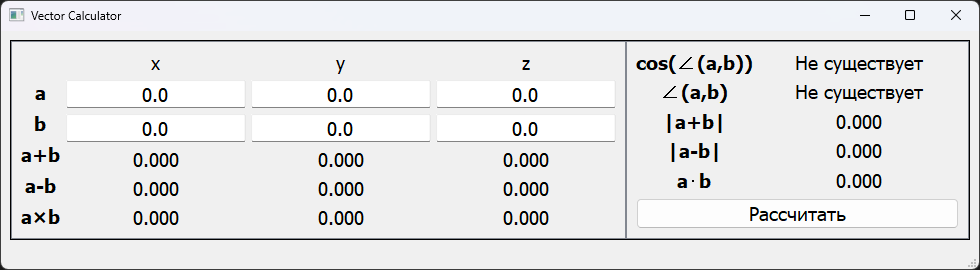
\includegraphics[width=\textwidth]{img//test1}
    \caption{}
\end{figure}

\begin{figure}[H]
    Пример с "египетским треугольником"
    \vspace{0.3cm}
    

    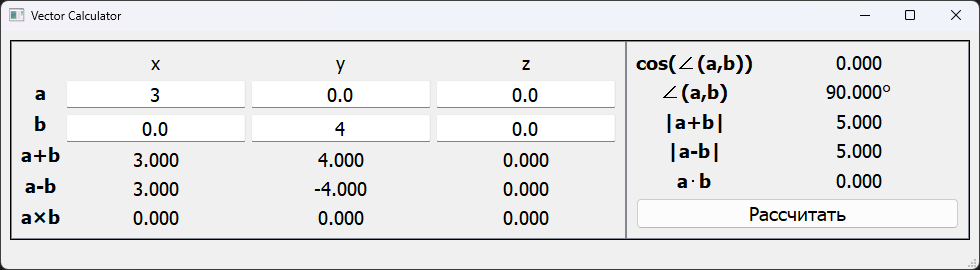
\includegraphics[width=\textwidth]{img//test2}
    \caption{}
\end{figure}

\begin{figure}[H]
    Пример с равнобедренным прямоугольным треугольником
    \vspace{0.3cm}
    

    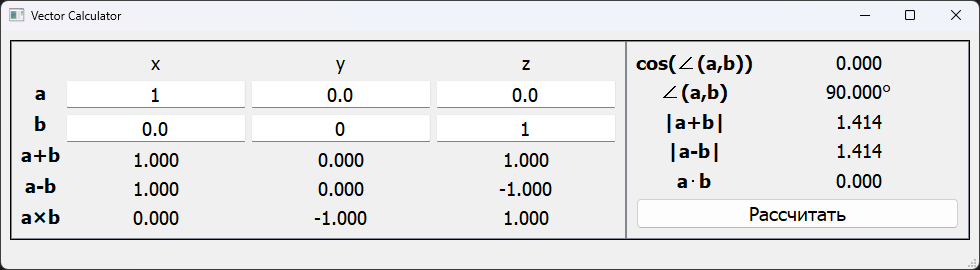
\includegraphics[width=\textwidth]{img//test3}
    \caption{}
\end{figure}

\begin{figure}[H]
    Пример с большими числами
    \vspace{0.3cm}
    

    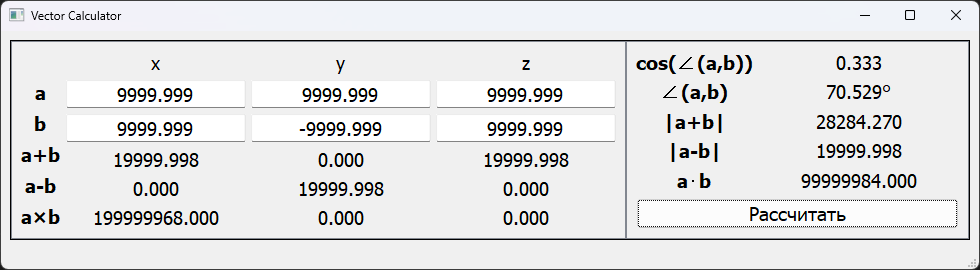
\includegraphics[width=\textwidth]{img//test4}
    \caption{}
\end{figure}

\end{document}